\section{Methodology}
\label{sec:methodology}
In this section, we will discuss the pipeline we follow to detect insecure patterns in code snippets as shown in Figure~\ref{fig:pipeline}. We will first discuss about repairing the code snippets (section ~\ref{subsec:code-repair}), and then converting the repaired to code snippets to an Intermidiate representation (IR) to run analysis (section~\ref{subsec:converting-to-IR}). Lastly we will finish by describing the techniques we have applied on the converted IR to detect the insecure patterns (section~\ref{subsec:identifying-insecure-patterns}), which we have previously described in section~\ref{sec:insecure-patterns}.     
\begin{figure*}[t]
  \centering
  \includegraphics*[width=0.8\linewidth]{Figures/overall-process.png}
  \caption{Overall processing pipleline of insecure pattern detection (1) collecting 1.6K code snippets from Stack Overflow, 
  (2) applying code repairs on collected code snippets, (3) converting code snippets to Jimple 3-address intermidate representation,
  (4) detecting 8 insecure most insecure patterns using keyword searching and backword flow analyis.}
  \label{fig:pipeline}
\end{figure*}


\subsection{Code Repair}
\label{subsec:code-repair}
% code snippets convey single intents
While writing code snippets as answers to posted questions, developers tend to be concise and short. The reason being long code snippets has lower chance of being accepted and upvoted by others in online platforms such as Stack Overflow.\fixme{Give a statistic on the avg. length of the code snippets of the dataset} Within a few lines of code, developers try to convey the intent hinting at a working solution by asuuming everything other are in place to for sucessful compilation. However this very mindset of developers can leave syntatic errors, missing classes in the code snippets. As a result, converting these code snippets to IR for analysis becomes difficult.

For identifying insecure patterns for which only keyword searching is sufficient (e.g., Rule 7, 8 as shown in Table~\ref{tab:keyword-searching}) this is not a problem since we don't need to convert them to any IR. However for idenitfying insecure pattern (e.g., Rule 1-6 as shown in Table~\ref{tab:slicing}) which requires running analysis this poses a problem. Therefore to identfy them, we need to add some repairs to the code snippets. For the purpose of this paper, we have applied the following repairs to the code snippets.

\subsubsection{Syntatic repair}
To remove the syntatic error present on the code snippets we do the following syntatic repairing.
  \begin{itemize}
    \item We remove illegal characters ( e.g., ``\&gt;'', ``\&lt;'', ``\&amp;'', ``\&quot;'' ``\&\#x27'', etc). Many of these illegal characters appered as the dataset was crawled from Stackoverflow website's raw HTML and HTML sanitizes some characters which are used in the code snippets. Also some code snippets have comments without any comment sign, and dots to implify some code would be here which not relevent to question posted.    
    \item Some code snippets do not have match brackets, and extra quotes for strings. 
    \item Some code snippets have \texttt{@Overide} notation implying it is implementing an interface. However the partial program analysis tool we will discuss to convert code snipeets to IR, can not handle \texttt{@Override} notation.
  \end{itemize}
     

\subsubsection{Missing package, class, and method names:}
Partial Program Analysis (PPA) tool which we have used to convert the code snippets to IR, can not consume a lines  of code missing classname, package name, method names. Therefore we applied the following repairs. 
\begin{itemize}
\item If the code snippet is missing any class name, we wrap the code snippet inside a public class name. If the code snippet already has a public class, we rename the file according to that public class.
\item If the code snippet does not have any package name, we place the public class in a package, and add the package name to the code snippet. If the code snippet has package name, we create proper directory strcuture according to the package name and place the code snippet there before converting them to IR. 
\item We also add dummy implementation of missing methods as developers tend to have methods names  in code snippets but does not give any implementation within the code snippets.
\item Finally, we load the some popular crypto classes in Java to the runtime of PPA tool which are imported, implemented by code snippets frequently. This helped us to avoid missing class name, unknown interface error thrown by PPA in many cases.  
 
\end{itemize}
       
\subsection{Converting code snippets to IR}
\label{subsec:converting-to-IR}

After repairing the code snippets, we tried to convert them to IR grammer named Jimple. Jimple~\cite{vallee1998jimple} is a 3-address intermediate representation that has been designed to simplify analysis. Jimple was inspired from SIMPLE an AST to represent C statements. To convert the code snippets we used a tool named partial program analysis (PPA). Dagenais et al. developed PPA ~\cite{dagenais2008enabling} with goal of analyzing only subset of a program source code which matches with our use case of analysing code snippets. PPA  can infer types where types are not present that subset of the code. In case of failure PPA will place special type \texttt{"MAGICCLASS"}, \texttt{"MAGICCLASS"}, and \texttt{"MAGICMETHOD"}. This is necessary since without types it is not possible to build the abstract syntax tree, and eventually convert the code snippet to Jimple for a strongly typed language such as Java. As PPA can overcome this problem by inferring types of the objects used in the subset of the program source code, it can convert the subset program source code. We leverage PPA after making the code repairs presented in previous subsection~\ref{subsec:code-repair}. Otherwise a large number of code snippets was throwing errors as PPA can not handle errounos code snippets.     

The idea is to feed the Jimple representation of the code snippet to Soot -- a state-of-the-art program analysis tool~\cite{soot}. Soot API can consume a Jimple representation, and perform data flow analysis which is as discussed in the next subsection~\ref{subsec:identifying-insecure-patterns}, required for detecting insecure patterns.
\iffalse
\minote{Talk about your choice of PPA}
\begin{itemize}
    \item Have used PPA. 
    \item Talk about Jimple / AST.
\end{itemize}
\minote{Add a number on how many code snippets you have been able to convert here..}
\fi

\subsection{Identifying insecure patterns}
\label{subsec:identifying-insecure-patterns}
In this subsection we will discuss the two techniques we have used to identify the insecure patterns discussed in section~\ref{sec:insecure-patterns}. Specifically we haved used two techniques found in the existing literature. One of them is keyword based detection, and the former one is using back flow sensitive analysis. 
\begin{table}[ht]
\scriptsize
  \begin{tabular}{|l|l|}
  \toprule
  \begin{tabular}[c]{@{}l@{}}Rule\\ No\end{tabular} & keywords  \\ \midrule 
  7                                                 &  \texttt{SSLSocketFactory.ALLOW\_ALL\_HOSTNAME\_VERIFIER} \\                                         
  8                                                 &  \texttt{*.csrf.disable()}                             \\ 
  \bottomrule
  \end{tabular}
  \caption{}
  \label{tab:keyword-searching}
\end{table}

\begin{table}[ht]
 %\resizebox{\linewidth}{!}{
   \scriptsize
  \begin{tabular}{|l|l|}
  \toprule
  \begin{tabular}[c]{@{}l@{}}Rule\\ No\end{tabular} & Slicing criteria       \\ \midrule 
  1 &  \texttt{KeyGenerator.getInstance(*)} \\    \midrule                                       
  2 &  \texttt{MessageDigest.getInstance(*);}      \\ \midrule 
  3 & \texttt{public void checkClientTrusted} \\
   & \texttt{public void checkServerTrusted} \\ 
  & \texttt{public X509Certificate[] getAcceptedIssuers()} \\ \midrule
  4 &  \texttt{keyPairGenerator.initialize(keySize);} \\ \midrule
  5 & \texttt{public boolean verify} \\ \midrule 
  6 &\texttt{new SecretKeySpec(keyBytes, "AES")} \\ 
   & \texttt{*.load(*.openStream(), new String(keyBytes).toCharArray());} \\
   &  \texttt{new PBEKeySpec(new String(keyBytes).toCharArray(),*);} \\
  \bottomrule
  \end{tabular}
  \caption{}
  \label{tab:slicing}
 %}
\end{table}

\subsubsection{Key word base analysis}
In keyword based analysis, we want to write an regex which can capture the common way developers write the insecure patterns, and then searching in the code snippets for matching the written code snippets. This method was used by Rahman et al.~\cite{akondsnakes} to detect insecure practices present in Python code snippets on Stackoverflow. Although being a simple technique, it worked surprising well for them i.e, does not introduce any false positives. However, in our case, as we will show in the next, that capturing all the insecure pattern by writing regex can introduce false-positives even simple code snippets.

Therefore, according to our manual observation, we can detect only two insecure patterns using keyword searching. This follows from the resoning that Rule 7 and 8 can be written by any developer, in the exact pattern as shown in Table~\ref{tab:keyword-searching}. For detecting the other 6 insecure patterns, we have to restore to backword flow program analysis as described next.  
%Since based on manual inspection, only these two insecure patterns detection can be captured by regex without introducing false positives. 
%Keyword based detection analysis as the name suggestion is writing regex for common way developers wrie 

\subsubsection{Backword flow base analysis.}
We use the backword flow analysis intrdocued by Rahaman et al.~\cite{cryptogurd} in their CryptoGurd Project. They introduced specialize def-use analysis~\cite{use-def} based on program slicing techniques~\cite{program-slicing} to detect 16 common cryptographic API misuses in Apache, and Android projects. Def-use  dataflow analysis builds a dependency relation based on the definition and use statements. Given a slicing criteria, which is a statement, or a parameters of an API, backword flow analysis computes the set of program statements that affects the slicing criteria in terms of data flow. The key design choice, hence, here is to specify special function invokation places as the slicing crteria. The slicing criteria used for paper are highlighted in Table~\ref{tab:slicing}. 

Now we will detail why simple keyword based analysis is not sufficient for detecting rules 1-6 as they can introduce FP even for simple rules. To demonstrate this, consider the example code snippet shown in listing~\ref{fig:aes-without-vars} corresponding to insecure pattern rule 2 -- detecting insecure broken cryptographic hashes MD5, MD4, MD2, SHA1. We can use keyword searching based technique on the name of broken hashes, and successsfully detect that the insecure pattern that code snippet in listing~\ref{fig:aes-without-vars} have used broken hash. However it will introduce Fasle positive for same insecure pattern on the code snippets shown in listing~\ref{fig:aes-without-vars}.% show a listing where MD5 is mentioned as commment, and overwritten as variable.
As there are multiple ways developers can use these broken hashes, unlike rule 7-8, we set \texttt{MessageDigest.getInstance(*);} as the slicing criteria. Then we start backword def-use analysis to see if any of the program sets affects the paramters of \texttt{MessageDigest.getInstance(*);}, and has a value of equal to name of the broken hash.


\begin{lstlisting}[caption={A code snippet where keyword based detection work well}, label={fig:aes-without-vars}]
    ...
    MessageDigest md = MessageDigest.getInstance("MD5");
    md.update(str.getBytes());
    ....
\end{lstlisting}

\begin{lstlisting}[caption={A code snippet where keyword based detection introduces FP}, label={fig:aes-with-vars}]
    ...
    int flag = 2;
    MessageDigest md = MessageDigest.getInstance("MD5");
    if(choice > 1){
       md = MessageDigest.getInstance("SHA-256");
    }
    md.update(str.getBytes());
    ....
\end{lstlisting}

\minote{A formal proof is given in the Appendix.}

We modified the code base of  as CryptoGuard\footnote{\url{https://github.com/CryptoGuardOSS/cryptoguard}} to achieve our analysis on code snippets. This is for two reasons. Firstly, CryptoGuard already has the basic skelection for use-def analysis, and we just have to change the slicing criteria. Secondly, CryptoGurd uses Soot as the underlying program analysis enginee. Hence we can provide our generated Jimple IR using the PPA tool to CryptoGuard, and   CryptoGurd's program analysis enginee Soot can do backword analysis based on the slicing criteria defined by us.

Figure~\ref{fig:slicing} shows one such example. Taking \texttt{SecretKeySpec} as the slicing criteria, we identify the set of statements which affects the first parameter of \texttt{SecretKeySpec} -- which is \texttt{MyDifficultPassw} here. Eventurally we will backtrack to the definition program set and can reason that it is randomly generated - rather a hard coded  secret. Since this makes the \texttt{SecretKeySpec} class object \texttt{sks} predictable, we have detected the presence of insecure pattern 6.

\begin{figure}[ht]
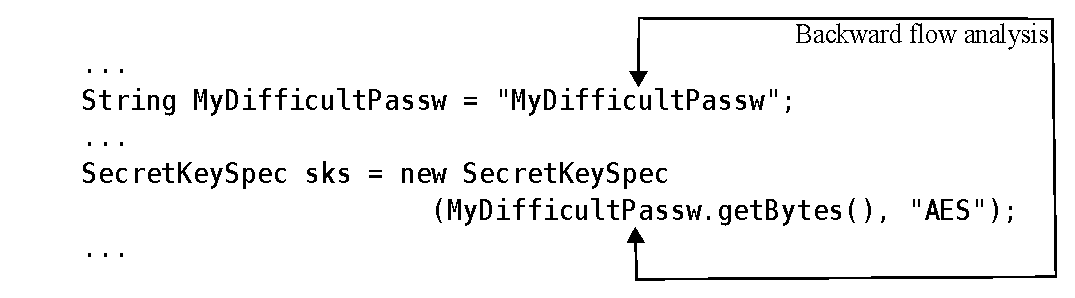
\includegraphics[width=\linewidth]{Figures/bckfwanalysis.eps}
\caption{}
\label{fig:slicing}
\end{figure}

%\minote{Here give one example explaining how you have choosen the slicing criteria, and the backword flow analysis. Then say example codes for other rules are given in the appendix}
%The backword flow analysis starts a def-use analysis from the specified special function invokation place.    
% Talk why keyword based analysis can find FP. Also it would be better to show one code snippet in the start and refer it throughout the paper.
% Wrtie the lemma here that why FP will introduce no FP if the FP is with the the same procedure.
% Wait I could have used CryptoGurd to detect the inseucre patterns.. right?  

%\subsection{Synthesizing secure patterns}